% v2-acmtog-sample.tex, dated March 7 2012
% This is a sample file for ACM Transactions on Graphics
%
% Compilation using 'acmtog.cls' - version 1.2 (March 2012), Aptara Inc.
% (c) 2010 Association for Computing Machinery (ACM)
%
% Questions/Suggestions/Feedback should be addressed to => "acmtexsupport@aptaracorp.com".
% Users can also go through the FAQs available on the journal's submission webpage.
%
% Steps to compile: latex, bibtex, latex latex
%
% For tracking purposes => this is v1.2 - March 2012
\documentclass{acmtog} % V1.2

%\acmVolume{VV}
%\acmNumber{N}
%\acmYear{YYYY}
%\acmMonth{Month}
%\acmArticleNum{XXX}
%\acmdoi{10.1145/XXXXXXX.YYYYYYY}

\acmVolume{}
\acmNumber{}
\acmYear{}
\acmMonth{}
\acmArticleNum{}
\acmdoi{}

\usepackage{listings}
\usepackage{color}
\begin{document}

\title{Classifying Malware into families Based on File Content} % title

\author{Patrick Rand {\upshape and} Reynier Ortiz
\affil{School of Computing and Information Sciences\\
Florida International University\\
Miami, Florida, USA}
}

\category{H.3.3}{Information systems}{Information retrieval}[Information Search and Retrieval]

\keywords{malware, classification, n-grams}

\maketitle

\begin{abstract}
\label{abstract}
\textbf{\emph{Abstract}}-- We present a mechanism to classify a malware file into
one of nine families: Rammit, Gatak, Tracur, Vundo, Simda, Kelihos\_ver1, Obfuscator.ACY,
Lollipop and Kelihos\_ver3. The system uses a large training set of disassembled malware executables, both in their binary and assembly forms. We ran two separate experiment processes: the first involved extracting n-grams from the binary files using the kfNgram tool, and the second used a Bash script to parse the assembly files for method calls to external API libraries. In both cases, the attributes s are merged to form a master
list and later reduced by selecting the top 500 with the highest information gain \emph{(IG)}.
These 500 attributes are the boolean attributes to determine if they are present or not in
each of the malware executables. The training set, using the selected attributes, was
transformed into an .arff file required by Weka \cite{weka} to run several classifiers, 
i.e. naïve bayes, decision trees and support vector machines (SVM). We then compared the
different algorithms using some common measures: accuracy, error rate, true and false positive 
error rates.
\end{abstract}

\section{Introduction}
\label{sec:intro}
In recent years, the malware industry has evolved into a complex industry, causing both severe personal and commercial damage. Traditional methods of malware detection typically involve matching a piece of malware to a signature, that has been predefined in the system. However, malware programmers have learned to evade signature detection by polymorphically obfuscating their code. What this means is that, for any given piece of malware, the program itself will be recompiled with randomized variable and string names, rendering standard signature detection near useless in identfiying a piece of malware. This has given rise to another goal of both research and industry: given a piece of malware, can we classify it into a common malware family, such that each instance of that family was morphed from the same original malware program. The ability to categorize a malicious program into a known family provides great importance because it allows for a more focused recovery and repair process .Despite this, researchers have developed methods for indetfiying malware by only considering static portions of the malcicious code that are unaffected by polymorphism. In particular, these attributes are the method calls of the external libraries used in the code, and the byte sequence of executable. While the research behind these evaluation processes have shown to have good results, much of this research was performed on small sample size of data, usually less than a few hunderd or a thousand exmaples. The small data sizes is most likely attributed to the difficulty involved with building a data set of malware. First, a program will need to be trapped and identified as malware. From there, researchers can examine the code either dynamically, or statically. The former involves tracing the program's execution in secure, virtual sandbox environment, while the latter involves running the program through a disassembler, and outputing its source code. This paper and its referenced work focus on static anaylisis of programs, which can be generalized into a form of text/document classification, of which there is extensive research in the machine learning community. The purpose of this paper will be to survey and examine previous research in the field, and evaluate how these methods scale and perform on a very large dataset. Microsoft has provided a sample dataset of 10,838 disassembled malware executables, of which each program is given in both its hexadecimal byte form, and its assembly form. Each of these training examples have been labeled as belonging of one of the aforementioned malware families. The results of our experiment showed similiar and at times slightly improved classification accuracy compared to preivous research. Also, our modified system, designed to handle our 400 GB training performed well and showed its ability to scale with the large data set. Given more time, we would have liked to explore how are system handles classifying both programs that do not belong to one of the 9 origin families, as well as those that are not malware. 


\section{Problem Definition and Methods }
\label{sec:problem_def}
%
\looseness-1

\subsection{Task Definition}
blah blah

\subsection{Algorithms and Methods}
Our approach to feature extraction and classification is based on a combination of the methods from the common text classifaction techiniques developed in previous research (cite). Where our process differed from these methods is our focus on the design of the entire system architecture, in particular, creating a system that was not only able to replicate the successful results of the referenced research, but to do so on a data set of substantially larger magnitude in size. The size of our training set required us to design the feature extraction process in a MapReduce-styled pattern (cite), but also to only consider machine learning classifiers that were able to scale with our large input. Thus, classifiers such as k-nearest-neighbors and Hidden Markov Models (cite) were not considered due to their performance on large data-sets and the impracticality of scaling them in regards to our limited computing resources. For both types of feature-sets, we evaluated the classification performance of three classifiers: Naive Bayes, Decision Trees, and Support Vector Machines. Of these classifiers, Decision Trees and Support Vector Machines performed best, and from there we extended our analysis into the boosted forms of these two algorithms. 

\subsubsection{System Architecture}
As shown in figure Fig \ref{fig:architecture}, the architecture of the system is rather simple. The main tasks were the
preprocessing of the data which involved extracting the N-grams and transform the
training set into a format that Weka \cite{weka} accepts as input. And then apply several
learning methods.

\begin{figure}
\centering
\scalebox{0.70}{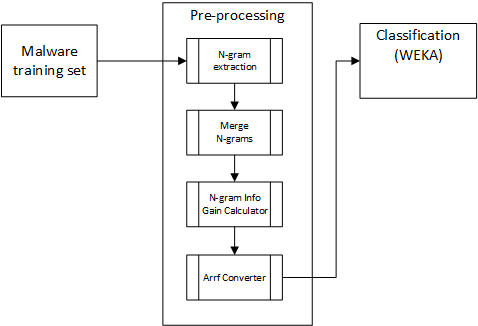
\includegraphics{system_architecture.png}}
\caption{System architecture.}
\label{fig:architecture}
\end{figure}

\subsubsection{Data Preprocessing}
The preprocessing part was a process that required a considerable effort because of the 
size of the training set, 10,868 files. The first step was to extract the hexadecimal
N-grams from the binary files using the kfNgram tool \cite{kfngram}, we used n=4.

It was then necessary to merge the resulting sorted N-gram files to effectively calculate the
\emph{information gain (IG)} of each N-gram. Because these files were extremely long,
we could not use the merge functionality built in the kfNgram tool, and we have to halt
the application after running for three days. To optimize this process we merged the files
maintaining a min-heap (or \emph{PriorityQueue} in Java) in memory with the first distinct N-gram 
from each file, as shown in Fig \ref{fig:merge_int}. We were also able to keep 10,878 Java
scanners in memory to speed up I/O. Then, to merging process would consist in each iteration
to perform a \texttt{pop()} operation from the \texttt{PriorityQueue}, append the element to merged
file, and insert the next N-gram from the same file of the element that was popped to the
\texttt{PriorityQueue}. This process is represented in Fig \ref{fig:merge_pop_replace}.

\begin{figure}
	\centering
	\scalebox{0.70}{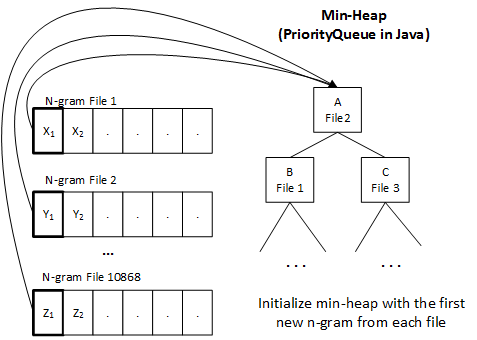
\includegraphics{merge_ngrams_init.png}}
	\caption{Initializing PriorityQueue to merge N-grams.}
	\label{fig:merge_int}
\end{figure}

\begin{figure*}[t]
	\centering
	\scalebox{0.70}{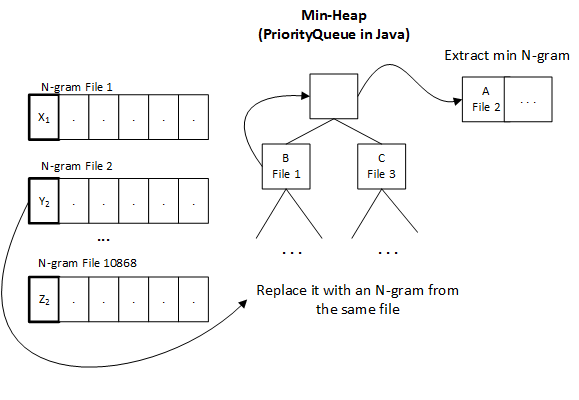
\includegraphics{merge_ngrams_pop_replace.png}}
	\caption{Process of merging N-grams. The minimum element is extracted and replaced with 
		another N-gram from the same file}
	\label{fig:merge_pop_replace}
\end{figure*}

Once merging was complete, we obtained a total of N-grams was 255,942,370, therefore we had to reduce 
them by calculating the  \emph{information gain (IG)} of each N-gram and selecting the top 500
(Fig. \ref{fig:info_gain_calc}), the same approach used in \cite{kolter:06}. The \emph{average mutual
information} \cite{yang:97} was used to select the most relevant attributes:

\begin{equation}
IG(j) = \sum_{v_j \in \{0,1\}} \sum_{C_i} P(v_j, C_i) \log \frac{P(v_j, C_i)}{P(v_j) P(C_i)}
\end{equation}

where \(C_i\) is the ith class,\(v_j\) is the value of the jth attribute, \(P(v_j, C_i)\) is the proportion that the jth
attribute has the value \(v_j\) in the class \(C_i\), \(P(v_j)\) is the proportion that the jth n-gram takes the value
\(v_j\) in the training data, and \(P(C_i)\) is the proportion of the training data belonging to the class \(C_i\) \cite{kolter:06}.

\begin{figure}
	\centering
	\scalebox{0.70}{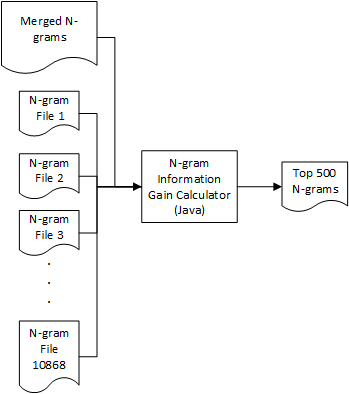
\includegraphics{N-gram_infogain.png}}
	\caption{Process of calculating the information gain of each N-gram.}
	\label{fig:info_gain_calc}
\end{figure}

The final step, as shown in Fig \ref{fig:ngram_arff}, in the data preprocessing was to transform the training set in .arff format where each example was represented by the presence (or absence) of the top 500 N-grams. This .arff file is one of the formats supported by Weka \cite{weka}, which facilitated to experiment with different machine learning algorithms.


\begin{figure}
	\centering
	\scalebox{0.65}{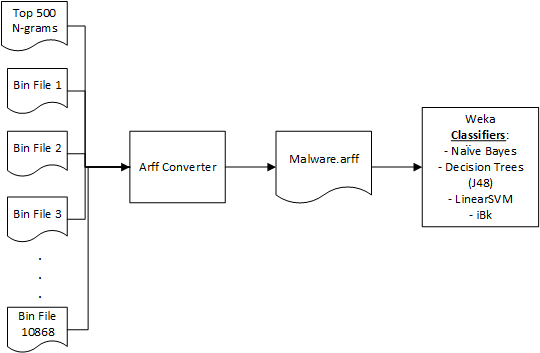
\includegraphics{n-gram_arff.png}}
	\caption{Transforming training set into .arff format.}
	\label{fig:info_gain_calc}
\end{figure}

\subsubsection{Classification algorithms}
\label{subsubsec:classif_alg}
1. Naive Bayes
	The Naive Bayes classifier uses Bayes' Theorem to label examples based on the assumption of conditional independence between features. Given a data set consisting of word counts, the training of this algorithm is very simple, and only requires the computation of the prior probability of each class, \(P(C_i)\), and the conditional probability of each word given a class, \(P(v_j|C_i)\). For a given instance \textbf{v}, we aim to classify it into some class, \(C_i\), thus computing \(P(C_i|v)\). Using Bayes' Theorem, this can be decomposed into:
\begin{equation}
P(C_i|\mathbf{v}) = \frac{P(C_i) \ P(\mathbf{v}|C_i)}{P(\mathbf{v})} 
\end{equation}	
We can ignore the \(P(\mathbf{v})\) term, and estimate the remaining feature probablitiles as:
\begin{equation}
P(C_i) = \frac{\textrm{\# of occurences of class \textit{i}}}{\textrm{\# of total attributes}} 
\end{equation}
\begin{equation}
P(v_j|C_i) = \frac{\textrm{\# of occurences of attribute } v_j \textrm{ with class }C_i}{\textrm{\# of occurences of class \textit{i}} }
\end{equation}
From here, we can define the classification of training example \textbf{v} as:
\begin{equation}
\hat{y} = argmax \ P(C_k) \displaystyle\prod_{i=1}^n p(v_i \vert C_k)
\end{equation}

2. Decision Tree
Decision trees are a method of classification that use tree-like graphs to model the classification of an example as a path of probabilites from the root node attribute, to one of the leaf (class) attributes. The beauty of decision trees lies in their simplicity and easy interpretation. Likewise, decision trees can be thought of as a "white-box" classification model, because once the tree has been built, the researchers can visualize and analyze each sub-path of an example's classification path.The basic implementation of a decision tree works as follows: for each node of tree, we select the attribute that best splits the our training examples into their respective classes. For our system, we used the J48 decision tree algorithm in Weka, which is an implementaion of the ID3 decision tree algorithm \cite{}. The algorithm is defined as follows:
1. Compute the entropy of each attribute in the data set S
2. Split the set S into subsets using the attribute for which entropy is minumim (or IG is max)
3. Make a decision tree node containing that attribute
4. Recur on subsets of remaining attributes

We define the entropy for a data set S, and its set of attributes V, as:
\begin{equation}
H(S) = - \sum_{v \in V} P(v) \log_{2} P(x)
\end{equation}
Once we obtain the corresponding decision tree, we prune the tree to help minimize over-fitting that may have occurred as a result of tree's greedy construction.


3. SVM  

\section{Experimental (and/or Theoretical) Evaluation}
\label{sec:evaluation}

\subsection{Methodology}
\label{subsec:methodology}
Blah blah 

\subsection{Results}
\label{subsec:results}
Blah blah \cite{WebGL:2014:Online}.

\subsection{Discussion}
\label{subsec:discussion}
Blah blah \cite{WebGL:2014:Online}.

\section{Related Work}
\label{sec:relatedwork}
%
Malware detection and classification is a problem being addressed through several angles. In \cite{oakland:2005}, 
the goal is to detect if a program exhibits a specified malicious behavior by determining if a set of templates of
sequence of instructions are present in the executable files. This approach requires to have knowledge on semantics
of each of the malware families. Although the results are promising, there are several reasons we could not follow
this approach, for example, as inferred by the title, it would be necessary to create a set of sequence of instructions
for each of the nine families we need to classify the malwares into. This is infeasible due to the length of the
course, but also it is outside of the scope of the course. As exhibited in the results, this strategy is resilient to
obfuscation and showed improvements when compared to McAfee VirusScan.

Several malware classification algorithms are based on n-grams extracted from the executable files. In \cite{securware:2011},
instead of byte sequences, the n-grams extracted are formed by machine codes. After obtaining the n-grams from the
malwares, a centroid for each family is created by selecting the most frequent n-grams. Then, the strategy to classify
a malware into one of the families, is to determine the centroid which the malware is more similar to by counting the
number of matching n-grams. When considering this approach, one of the possible limitations analyzed was that selecting
the most frequent n-gram could implicate choosing an n-gram irrelevant to the malware family.

We also explored sequential pattern extraction of n-grams. The proposed methodology in \cite{liangboonprakong:2013} 
outlines a procedure to use the n-grams patterns to classify the malware by family. The kfNgram tool \cite{kfngram} was
used to extract the n-grams from the disassembled files with n=1, n=2, n=3 and n=4, obtaining the best results with n=4. 
In \cite{kolter:06} the accuracy achieved was higher with n=4, therefore we skipped this evaluation and use only 
n-grams with n=4. The sequential pattern extraction technique in \cite{zhong:2012} was used to generate frequently 
occurred sequences of n-grams to represent the data \cite{liangboonprakong:2013}. Then the patterns significance 
was calculated using the term frequency-inverse document frequency (TF-IDF) where the term refers to the n-gram 
pattern and a document to the malware file. Since the number of patterns was too large, the sequential floating 
forward selection (SFFS) procedure was applied to reduce the number of features, in this case, n-gram sequential 
patterns. With all the features extracted, three classification algorithms were used, C4.5, multilayer perceptron 
and support vector machine. The training set was randomly split into two partitions using 80\% for training and 
20\% for testing achieving a 96.64\% of accuracy  \cite{liangboonprakong:2013}. Because of the duration of the 
course and the complexity of sequential pattern extraction, we were not able to experiment with this approach.

Following Occam's razor, suggesting that the simplest hypothesis is the best, we applied an approach similar to 
the one described in \cite{kolter:06}. The n-grams extracted from the executable files represented boolean features, 
present (i.e., 1) or absent (i.e., 0). Since the n-grams list was too large, it was necessary to select the most
relevant attributes (i.e., n-grams) by computing the \emph{information gain (IG)} described in \cite{yang:97} 
for each, also called \emph{average mutual information}. Through pilot studies, it was determined to use the 
top 500 n-grams, and then applied classifiers implemented in the Wakaito Environment for Knowledge Acquisition (WEKA) 
\cite{weka}: IBk, Naïve Bayes, SVM, and J48 (decision tree), and also \emph{boosted} the last three of these
 learners \cite{kolter:06}. The results indicated 98\% the highest accuracy using boosted decision trees.


\begin{lstlisting}
// Using ThreeJS, load character and 
// hair into mesh1 and mesh2 respectively

var hapgl = HapGL.init({ 
	ttsUrl: 'http://localhost:88/',
	character: mesh1,
	hair: mesh2
});
\end{lstlisting}

%
Generating emotions in HapGL was done also in the same manner as in HapFACS.
Emotion FACS (EmFACS) introduces a mapping of subsets of action units to
universal emotion identified by Ekman \cite{Ekman:1983} namely fear, anger,
surprise, disgust, sadness, and happines. The emotions implemented in HapGL
were:
\begin{itemize}
\item Happines, combining AU6, AU12, and AU25
\item Sadness, combining AU1, AU4, and AU15
\item Surprise, combining AU1, AU2, AU26, and AU5
\item Anger, combining AU4, AU5, AU7, AU23, and AU24
\item Disgust, combining AU9, AU15, and AU16
\end{itemize}

\texttt{getVoices(function getVoicesCallback)} returns a JSON object with an 
array of voices and will immediately call the \texttt{getVoicesCallback} function with
the result. Since the HapGLService uses Microsoft Speech API (SAPI), the voices are
SAPI-compatible installed on the web-server. More sophisticated voices can be
purchased and installed separately. The following is an example 
of the result of calling \texttt{getVoices}: 

\begin{lstlisting}
hapgl.getVoices(function(output) {...});

// Example of voices returned
{
   voices : [{
      id : "MS-Anna-1033-20-DSK",
      age : "Adult",
      name : "Microsoft Anna",
      gender : "Female",
      culture : "en-US"
   }]
}
\end{lstlisting}

\texttt{speak} and \texttt{speakssml} are similar, the only difference is that
\texttt{speak} will only accept a plain string, whereas \texttt{speakssml} can
accept a string in SSML format as input \cite{SSML:Online}. The \texttt{voice} parameter corresponds
to the \emph{name} attribute of the voices returned by \texttt{getVoices}, if no
\texttt{voice} is passed in then the HapGLService will synthesize using the default
voice in the TTS Server. The \emph{ssml} string argument for the \texttt{speakssml()} function
should be a well-formed SSML Version 1.0 \cite{SSML:Online}. SSML allows
to manipulate the voices by modifying parameters such as: \emph{volume}, \emph{rate},
and \emph{pitch} in the \texttt{<prosody>} elements. Several \texttt{<prosody>} elements
can be combined to produce the desired pronunciation of sentences.

The output of \texttt{speak(..)} and \texttt{speakssml(..)} contains the necessary
information to render the sequence of viseme transitions synchronized with the audio
stream to produce a realistic talking virtual human. The following example shows the
output when speaking the word ``Hello".

\begin{lstlisting}
hapgl.speak(``Hello");

// The output of speaking ``Hello"
{
    audioFormat: ``data:audio\/wav;base64",
    audioStream: ``...",
    visemes: [{
       number : 0,   // silence
       audioPosition : 0.0,
       duration : 3.0,
       emphasis : 0
   }
}
\end{lstlisting}

The sequence of visemes is already sorted in the correct order to be animated. All this
information is sufficient for the lip-synchronization algorithm to render each viseme
at the correct time. The viseme transitions are done smoothly, otherwise, just displaying
the viseme in its maximum intensity would create an undesired illusion. Each 
viseme transition takes a pair of visemes $V_0$ and $V_1$, where $V_0$ is the starting
viseme and $V_1$ is the ending viseme. To do the transformation $V_0 \rightarrow V_1$ we
consider the duration $d_0$ of $V_0$. In $d_0$ time, $V_0$ ``fades out" and $V_1$
``fades in". By ``fade out" we mean interpolating from $V_0$ by setting the value of the
corresponding morph gradually from 1 to 0 in $d_0$ time. Conversely, ``fade in" means
interpolating to $V_1$ by setting the value from 0 to 1. Each viseme maps to a corresponding 
phoneme, we use the mapping provided by the Microsoft Speech API as seen in 
Table \ref{tab:VisemeMapping}. 

\begin{table}[h]
\tbl{Viseme to phonemes mapping in Microsoft Speech API}{%
\begin{tabular}{|l|l|l|l|}\hline
Viseme &{Phoneme(s)} & {Viseme} & {Phoneme(s)}\\
\hline
0 & silence & 11 & ay \\
1 & ae, ax, ah & 12 & h \\
2 & aa & 13 & r  \\
3 & ao & 14 & l \\
4 & ey, eh, uh & 15 & s, z \\
5 & er & 16 & sh, ch, jh, zh \\
6 & y, iy, ih, ix & 17 & th, dh \\
7 & w, uw & 18 & f, v \\
8 & ow & 19 & d, t, n \\
9 & aw & 20 & k, g, ng \\
10 & oy & 21 & p, b, m \\
\hline
\end{tabular}}
\end{table}

Since not all the phonemes have its corresponding Haptek morph register, we choose 
the most similar morph. We used the following viseme to morph mapping in HapGL:

\begin{lstlisting}
var visemeMorphMapping = {
  `0': {name: `neutral'}, `11': {name: `aa'},
  `1': { name: `aa' }, `12': { name: `ih' },
  `2': { name: `aa' }, `13': { name: `n' },
  `3': { name: `aa' }, `14': { name: `n' },
  `4': { name: `ey' }, `15': { name: `s' },
  `5': { name: `er' }, `16': { name: `ch' },
  `6': { name: `ih' }, `17': { name: `th' },
  `7': { name: `uw' }, `18': { name: `f' },
  `8': { name: `ow' }, `19': { name: `d' },
  `9': { name: `aa' }, `20': { name: `g' },
 `10': { name: `ow' }, `21': { name: `m' }	
};
\end{lstlisting}

\begin{table}[h]
\tbl{AUs with recognition rate of less than 100\%. Taken from HapFACS \cite{hapfacs:2013}.}{%
\begin{tabular}{|l|c|l|c|}\hline
AU &{Recognition Rate} & {AU} & {Recognition Rate}\\
\hline
10 & 66.67\% & 16 & 33.33\% \\
11 & 66.67\% & 20 & 66.67\% \\
12 & 66.67\% & 23 & 33.33\%  \\
13 & 66.67\% & 25 & 33.33\% \\
14 & 66.67\% & 28 & 33.33\% \\
\hline
\end{tabular}}
\end{table}

\begin{table}[h]
\tbl{AUs comparisson between HapGL and HapFACS.}{%
\begin{tabular}{|l|c|c|}\hline
AU & {HapGL} & {HapFACS}\\
\hline
AU1 & 
\begin{minipage}{.18\textwidth}
  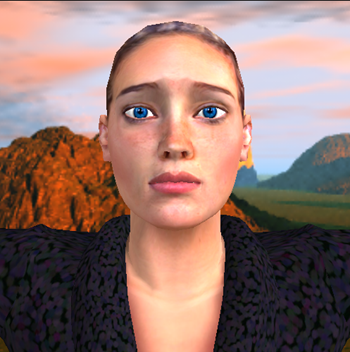
\includegraphics[width=\linewidth]{AU1_100}
\end{minipage}
& 
\begin{minipage}{.18\textwidth}
  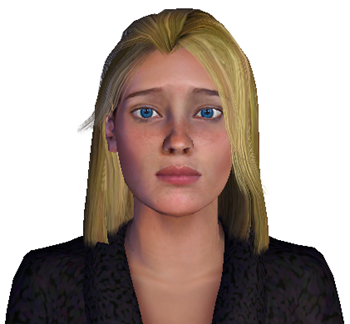
\includegraphics[width=\linewidth]{hp_AU1_100}
\end{minipage} \\
\hline
\end{tabular}}
\end{table}

\section{Future Work}
\label{sec:futurework}
Malware classification is a topic that is always evolving because viruses' 
authors are constantly developing techniques to avoid been detected, for 
example by obfuscating the code or by designing polymorphic behaviours. The 
proposed approach is agnostic of these techniques, therefore, we assume 
intuitively that a set of the extracted N-grams are product of this ingenious
methods. Mutation engines are capable of generating millions of variations of
the same virus, therefore, to overcome this problem, it would be necessary to
have knowledge of the malware behaviors to develop heuristics or detect specific
sequence of instructions to find in the malicious files.

For time reasons, we could not research on the possibilities of removing the
irrelevant computations in the malware files created to evade anti-viruses. This
would help, if using sequential N-gram patterns extraction, to detect patterns that
are truly correlated to the malware family. These patterns could, somewhat, describe
the common semantics present in each class of malwares.

\section{Conclusion}
\label{sec:conclusion}
%

Nevertheless, HapGL is still far from being used in production systems as it lacks of other necessary 
functionalities which could be part of future works. To name some, and not intended to be a comprehensive list,
we suggest the following:

\begin{itemize}
\item \emph{Detailed Evaluation}, due to time constraints, a thorough evaluation could not be performed. We suggest
to measure the \emph{believability} of the system by surveying a random sample of users, preferably greater than 20.
Although this is a subjective measure, a user study is still a good indication about the quality of the system.
\end{itemize}

% Bibliography
\bibliographystyle{ACM-Reference-Format-Journals}
\bibliography{malware-bibfile}

\end{document}
% End of v2-acmtog-sample.tex (March 2012) - Gerry Murray, ACM
